\documentclass[a4paper,12pt]{article}
\usepackage[french]{babel}
\usepackage[utf8]{inputenc}
\usepackage[T1]{fontenc}
\usepackage{mathptmx}
\usepackage{graphicx}
\usepackage{geometry}
\usepackage{amsmath}
\usepackage{float}
\usepackage{listings}
\usepackage{xcolor}
\usepackage{hyperref}
\usepackage{subcaption}
\usepackage{biblatex}

\setcounter{secnumdepth}{0}
\hypersetup{colorlinks=true, linkcolor=black}
\geometry{margin=1in}

\definecolor{codegreen}{rgb}{0,0.5,0.07}
\definecolor{codeblue}{rgb}{0.05,0,1.0}
\definecolor{codepurple}{rgb}{0.65,0.35,0.96}
\lstdefinestyle{mystyle}{
    commentstyle=\color{codegreen},
    keywordstyle=\color{codeblue},
    stringstyle=\color{codepurple},
    basicstyle=\fontfamily{pcr}\normalsize,
    breakatwhitespace=true,
    breaklines=true,
    frame=lines,
}
\lstset{style=mystyle}

\captionsetup{font={
    footnotesize,
    color=gray
}}

\addbibresource{img/references.bib}



\begin{document}
    \selectlanguage{french}
    
    \begin{titlepage}
        \begin{center}
            % Logo de l'école en en-tête
            
\includegraphics[width=5cm]{./img/uqac.png}\\[1cm]
            
            % Titre principal
            \vspace*{1cm} % Ajuster pour centrer verticalement
            {\Huge \textbf{Interaction Humain-Robot : Devoir 2}\\[0.5cm]}
    
            % Image de couverture (centrée en dessous du logo)
            \vspace*{1cm}
            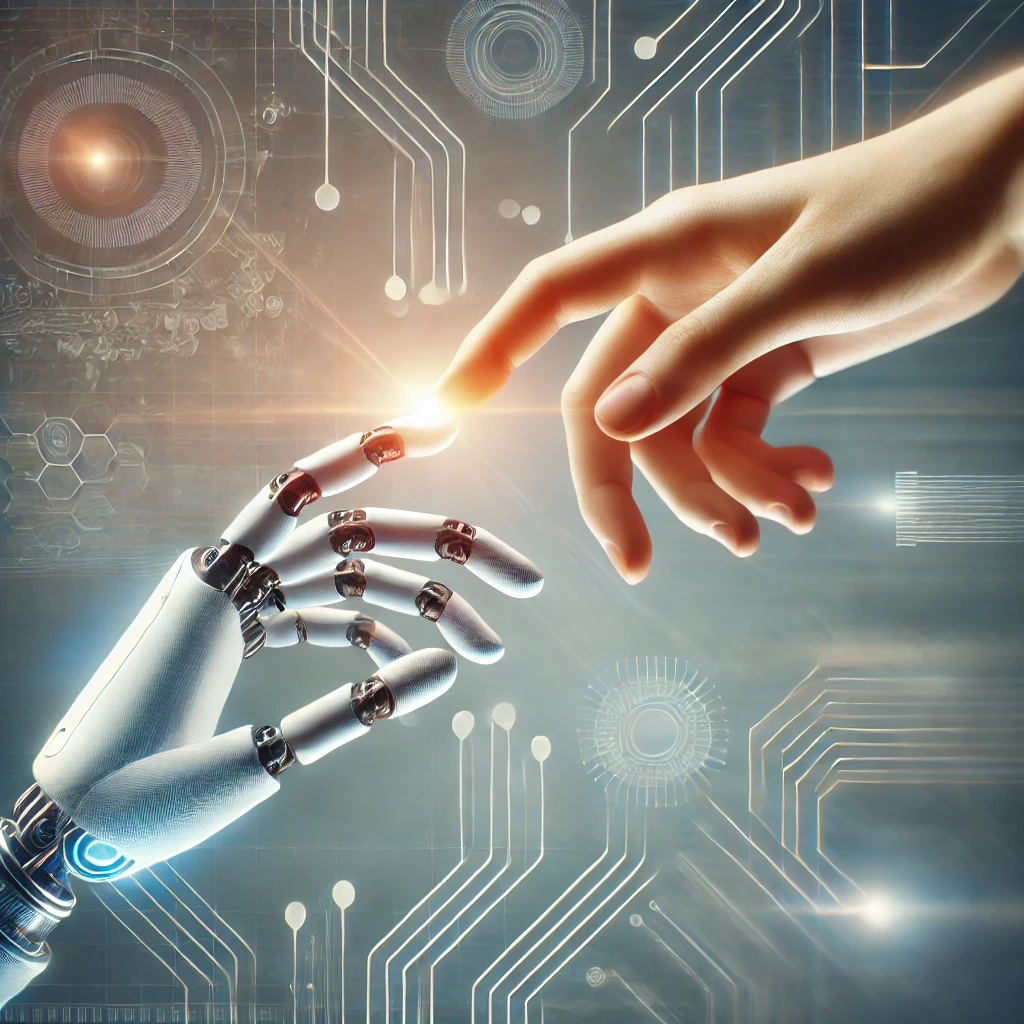
\includegraphics[width=0.7\textwidth]{./img/image_IHR.png}\\[1cm]
    
            \vspace{4.5cm}
            \begin{tabular*}{1\linewidth}{@{\extracolsep{\fill}}l c r}
                {\small Constance ALOYAU} &  & {\small ALOC25530200} \\
                {\small Erwan MAWART} & {\normalsize 16 novembre 2024} & {\small MAWE14050200} \\
                {\small Benjamin PELLIEUX} &  & {\small PELB28120100} \\
            \end{tabular*}
            
            \vfill
        \end{center}
    \end{titlepage}
    
    \tableofcontents
    \newpage
    \listoffigures
    \listoftables
    \newpage
    
    \section{Introduction}
    Les vibrations présentes dans un mécanisme robotique manipulé par un opérateur humain peuvent affecter de manière significative la précision et la qualité des tâches réalisées. Ces vibrations, générée notamment par la force que l'humain exerce sur l'interface de commande, peuvent devenir problématiques, notamment lorsqu’elles sont amplifiées par les mouvements involontaires ou l'ajustement de la rigidité du bras de l'opérateur. L'interaction entre l'humain et la machine crée ainsi un système complexe où les propriétés mécaniques du robot et de l’opérateur se superposent, entraînant des oscillations et perturbations indésirables. Ces vibrations ne nuisent pas seulement à la performance du système en altérant la précision des actions exécutées, mais elles peuvent également compromettre le confort de l'utilisateur et, à terme, affecter sa santé, en provoquant des tensions musculaires ou des troubles liés aux mouvements répétitifs.

    Dans ce contexte, cette étude se propose d'analyser et  de compenser ces vibrations. Notre approche repose sur le développement d’un observateur capable de détecter et de compenser efficacement l'impact des vibrations générées par les forces et mouvements de l’opérateur. En intégrant un modèle dynamique de la rigidité humaine dans la boucle d'asservissement, nous visons à réduire les effets indésirables de ces vibrations sur la qualité de la tâche réalisée. L’objectif étant de proposer une solution technologique qui permette d’améliorer la précision et le confort de l’utilisateur tout en garantissant une interaction harmonieuse entre le robot et son opérateur.

    
    \newpage
    \section{Énoncé 1 : Conception du modèle du mécanisme}
    \subsection{Question 1.1}
    \begin{figure}[H]
        \centering
        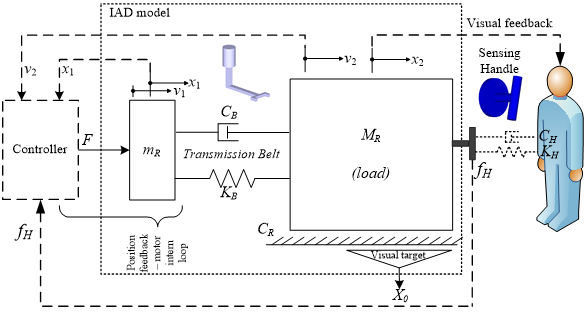
\includegraphics[width=14cm]{./img/modele_humain-meca_robotique.png}
        \caption{
            Modèle du mécanisme robotique et de l'humain \cite{Article1} \cite{Article2}
            \label{fig:ModelMecaRobotHumain}
        }
    \end{figure}
    
    La \autoref{fig:ModelMecaRobotHumain} présente le mécanisme robotique que nous allons utiliser, où :
    \begin{itemize}
        \item[$\bullet$] $M_R$ : masse de la charge \textit{[kg]}.
        \item[$\bullet$] $m_R$ : masse du système \textit{[kg]}.
        \item[$\bullet$] $K_B$ : constante de raideur des courroies \textit{[N/m]}.
        \item[$\bullet$] $C_B$ : coefficient d'amortissement des courroies \textit{[$N\cdot s/m$]}.
        \item[$\bullet$] $K_H$ : coefficient de raideur de l'humain\textit{[N/m]}.
        \item[$\bullet$] $C_H$ : coefficient d'amortissement de l'humain \textit{[$N\cdot s/m$]}.
        \item[$\bullet$] $C_R$ : coefficient de frottement \textit{[$N\cdot s/m$]}.
        \item[$\bullet$] $F$ : Force commandée par le système \textit{[N]}.
        \item[$\bullet$] $f_H$ : Force appliquée par l'humain \textit{[N]}.
        \item[$\bullet$] $x_1$ : position des moteurs \textit{[m]}.
        \item[$\bullet$] $x_2$ : position de la charge \textit{[m]}.
        \item[$\bullet$] $v_1$ : vitesse des moteurs \textit{[m/s]}, la dérivée de la position ($v_1 = \dot{x_1}$).
        \item[$\bullet$] $v_2$ : vitesse de la charge \textit{[m/s]}, la dérivée de la position ($v_2 = \dot{x_2}$).
    \end{itemize}
    
    Ainsi, on déduit les variables d'états ci-dessous.
    \[
        X =
        \begin{bmatrix}
            x_1 \\
            x_2 \\
            v_1 \\
            v_2
        \end{bmatrix}
        =
        \begin{bmatrix}
            x_1 \\
            x_2 \\
            \dot{x_1} \\
            \dot{x_2}
        \end{bmatrix}
    \]
    
    En effectuant la somme des forces appliquées sur chaque masse, on obtient le système suivant.
    \[
        \begin{cases}
            \sum F_{ext/m_R} = m_R\ddot{x_1} \\
            \sum F_{ext/M_R} = M_R\ddot{x_2} \\
        \end{cases}
        \Leftrightarrow
        \begin{cases}
            m_R\ddot{x_1} = F - K_B x_1 + K_B x_2 - C_B \dot{x_1} + C_B\dot{x_2} \\
            M_R\ddot{x_2} = K_B x_1 - K_B x_2 + C_B \dot{x_1} - C_B\dot{x_2} - C_R \dot{x_2} \\
        \end{cases}
    \]
    
    \begin{equation}
        \\ \Leftrightarrow
        \begin{cases}
            \ddot{x_1} = \frac{F - K_B x_1 + K_B x_2 - C_B \dot{x_1} + C_B \dot{x_2}}{m_R} \\
            \ddot{x_2} = \frac{K_B x_1 - K_B x_2 + C_B \dot{x_1} - C_B \dot{x_2} - C_R \dot{x_2}}{M_R}
        \end{cases}
        \label{eq:SommeDesForces}
    \end{equation}
    
    Grâce à celle-ci, on construit les deux équations de fonctionnement du système :
    
    \begin{equation}
        \dot{X}=AX+BU
        \Leftrightarrow
        \begin{bmatrix}
            \dot{x_1}\\
            \dot{x_2}\\
            \ddot{x_1}\\
            \ddot{x_2}
        \end{bmatrix}
        =
        \begin{bmatrix}
            0 & 0 & 1 & 0\\
            0 & 0 & 0 & 1\\
            \frac{-K_B}{m_R} & \frac{K_B}{m_R} & \frac{-C_B}{m_R} & \frac{C_B}{m_R}\\
            \frac{K_B}{M_R} & \frac{-K_B}{M_R} & \frac{C_B}{M_R} & \frac{-(C_B+C_R)}{M_R}\\
        \end{bmatrix}
        \begin{bmatrix}
            x_1\\
            x_2\\
            \dot{x_1}\\
            \dot{x_2}
        \end{bmatrix}
        +
        \begin{bmatrix}
            0\\
            0\\
            \frac{1}{m_R}\\
            0
        \end{bmatrix}
        \cdot F
        \label{eq:VarEtatXDot}
    \end{equation}
    
    \begin{equation}
        Y=CX+DU
        \Leftrightarrow
        Y=CX
        \Leftrightarrow
        \begin{bmatrix}
            x_2\\
            \dot{x_1}
        \end{bmatrix}
        =
        \begin{bmatrix}
            0 & 1 & 0 & 0\\
            0 & 0 & 1 & 0
        \end{bmatrix}
        \begin{bmatrix}
            x_1\\
            x_2\\
            \dot{x_1}\\
            \dot{x_2}
        \end{bmatrix}\\
        \label{eq:VarEtatY}
    \end{equation}
    
    L'\autoref{eq:VarEtatY} présente la sortie du système. Dans notre cas, on utilise $x_2$ (la position de la charge) et $v_1$ (la vitesse des moteurs) afin d'asservir notre système. Où $x_2$ permet à l'humain de corriger la trajectoire de la charge et $v_1$ d'asservir les moteurs.
    
    
    \subsection{Question 1.2}
    Lors d'une étude précédente, nous nous penchions sur la détectection des vibrations générées par le système lorsque l'humain se régédifie. Pour cela, nous analysions la vitesse des moteurs pour en extraire des caractéristiques temporelles et/ou fréquentielles qui nous permettent de déterminer la présence des vibrations. \\
    
    \begin{figure}[H]
        \centering
        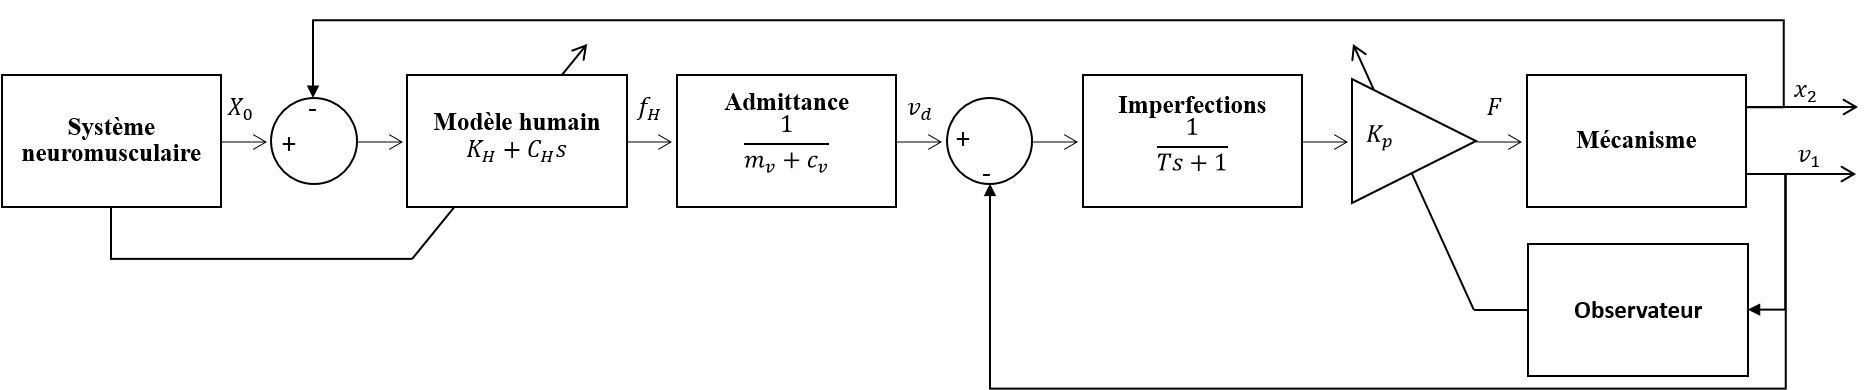
\includegraphics[width=16cm]{./img/SchemaBlocAvecObs.png}
        \caption{Commande des mécanisme robotique et humain avec observateur\label{fig:SchemaBlocAvecObs}}
    \end{figure}
    
    Afin de rendre le système autonome, il est donc nécessaire de rendre automatique cette recherche de caractéristiques. C'est pourquoi, comme le montre la \autoref{fig:SchemaBlocAvecObs}, on ajoute un observateur qui va influer sur la valeur du gain $K_p$, et donc, limiter les vibrations générées par le système.
    
    Dans Simulink, on représentera ce bloc avec l'architecture et la fonction contenues dans l'\hyperref[Annexe:modelObs]{annexe 7}.
    
    
    \subsection{Question 1.3}
    Le critère de Routh-Hurwitz est une méthode mathématique permettant déterminer rapidement la stabilité d'un système. Elle consiste à générer un tableau à partir des coefficients du dénominateur de la fonction de transfert tel que présenté au \autoref{tab:table_theo_critRH}. Une fois construit, on observe sa première colonne. Le nombre de changement de signe détermine la quantité de racines étant dans la partie astable du plan-s (c'est-à-dire dans la partie réel positive).
    
    \begin{table}[ht]
        \centering
        \[
        \begin{array}{|c|c c c c|}
            \hline
            s^n & a_n & a_{n-2} & a_{n-4} & \dots \\
            \hline
            s^{n-1} & a_{n-1} & a_{n-3} & a_{n-5} & \dots \\
            \hline
            s^{n-2} & b_{n-1} & b_{n-3} & b_{n-5} & \dots \\
            \hline
            s^{n-3} & c_{n-1} & c_{n-3} & c_{n-5} & \dots \\
            \hline
            \vdots & \vdots & \vdots & \vdots & \vdots \\
            \hline
            s^0 & h_{n-1} & h_{n-3} & h_{n-5} & \dots \\
            \hline
        \end{array}
        \]
        \caption{Tableau théorique du critère de Routh-Hurwitz}
        \label{tab:table_theo_critRH}
    \end{table}
    
    Dans le \autoref{tab:table_theo_critRH}, on retrouve :
    \begin{itemize}
        \item[$\bullet$] $a_{n-i}$, les coefficients du dénominateur.
        \item[$\bullet$] $b_{n-i}$, donnés par :
            $b_{n-i} = \frac{-1}{a_{n-1}}
            \begin{vmatrix}
                a_n & a_{n-i-1} \\
                a_{n-1} & a_{n-i-2}
            \end{vmatrix}
            = \frac{a_{n-1} a_{n-i-1} - a_n a_{n-i-2}}{a_{n-1}}$
        \item[$\bullet$] $c_{n-i}$, donnés par :
            $c_{n-i} = \frac{-1}{b_{n-1}}
            \begin{vmatrix}
                a_n & a_{n-i-2} \\
                b_{n-1} & b_{n-i-2}
            \end{vmatrix}
            = \frac{b_{n-1} a_{n-i-2} - a_n b_{n-i-2}}{b_{n-1}}$
        \item[$\bullet$] etc.
    \end{itemize} 
    
    On utilise cette méthode afin de déterminer la plage de valeurs des gain $K_p$. Afin de construire cette table plus simplement, on utilise cette fonction dans Matlab : \\
    \begin{lstlisting}[label={code:fctCritRH}, caption={Fonction Matlab génération du critère de Routh-Hurwitz}, language=Matlab]
    %%%%%%%%%%%%%%%%%%%%%%%%%%%%%%%%%%%%%%%%%%%%%%%%%%%%%%%
    % Parametres :                                        %
    %   - TF : la fonction de transfert a analyser        %
    %   - Oldvars : les variables a remplacer             %
    %   - Newvars : les valeurs a implementer             %
    %   - s : la variable de Laplace                      %
    % Sortie :                                            %
    %   - S : le tableau construit                        %
    %%%%%%%%%%%%%%%%%%%%%%%%%%%%%%%%%%%%%%%%%%%%%%%%%%%%%%%
    function S = calcTabRH(TF, Oldvars,  Newvars, s)
        % Extraction des coefficients du denominateur =====
        [~, Den] = numden(TF);
        [an, terms] = coeffs(Den, s);
        l_terms = length(terms);
        l = round(l_terms/2);

        % Creation du tableau =============================
        S = sym(zeros(l_terms, l));
        % Ajout des coefficients du denominateur
        for n=1:l
            i = n*2;
            S(l_terms, n) = an(i-1);
            if i < l_terms
                S(l_terms-1, n) = an(i);
            end
        end
        % Calcul des autres elements du tableau
        for k=l_terms-2:-1:1
            for n=1:l-1
                S(k, n) = (S(k+1, 1)*S(k+2, n+1)-S(k+2, 1)*S(k+1, n+1))/S(k+1, 1);
            end
        end

        % Remplacement des valeurs connues ================
        S = simplify(subs(S, Oldvars, Newvars));

        % Affichage du tableau ============================
        disp("Tableau du critere de Routh-Hurwitz :")
        disp(S)
    end
    \end{lstlisting}

    Les gains $K_p$ et $K_H$ étant dépendants l'un de l'autre, leur plage de valeurs varie en fonction de l'autre. Par conséquent, il nous est obligatoire de fixer l'un des deux. Ici, fixons $K_H = 50 N/m$, s'assurant ainsi la stabilité du système.
    
    En utilisant les valeurs données en \hyperref[Annexe:ValList]{annexe 1} dans le tableau du critère de Routh-Hurwitz, on obtient donc cinq coefficients contenant $K_p$. Parmis ceux-ci, le critère $S^2$ devient négatif à $K_p = 90$, comme présenté à la \autoref{fig:CoefS2}. Ainsi, on déduit que $K_p \in \left< 0, 90 \right>$.
    \begin{figure}[H]
        \centering
        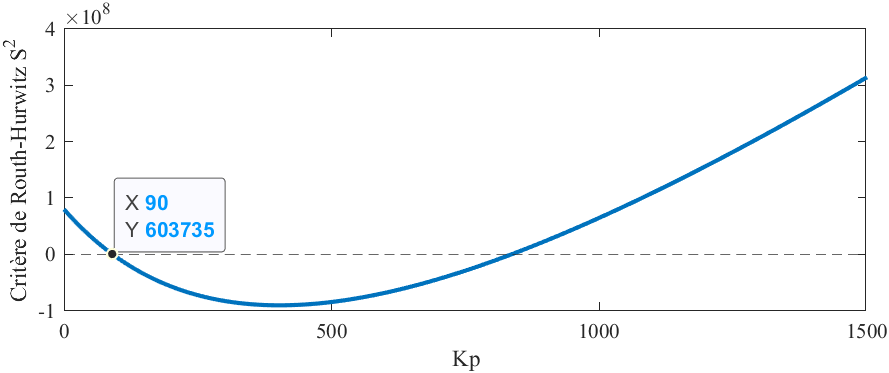
\includegraphics[width=16cm]{./img/plage_coefKp.png}
        \caption{Critère de Routh-Hurwitz $S^2$ en fonction de $K_p$\label{fig:CoefS2}}
    \end{figure}

    Afin de confirmer cette valeur, nous pouvons utiliser le lieu des racines. Cette méthode consiste à faire varier un gain en entrée du système afin de déterminer le moment auquel ce-dernier devient astable.
    
    Dans notre cas, le gain variable est $K_H$ et on fixe $K_p = 90$, condition limite déterminée à la \autoref{fig:CoefS2}. En traçant le lieu des racines, comme montré à la \autoref{fig:LieuRacineKh}, on remarque que le système est stable jusqu'à $K_H \approx 50$ ($K_H = 46.9532$ au point de mesure noté sur la \autoref{fig:LieuRacineKh}).
    \begin{figure}[H]
        \centering
        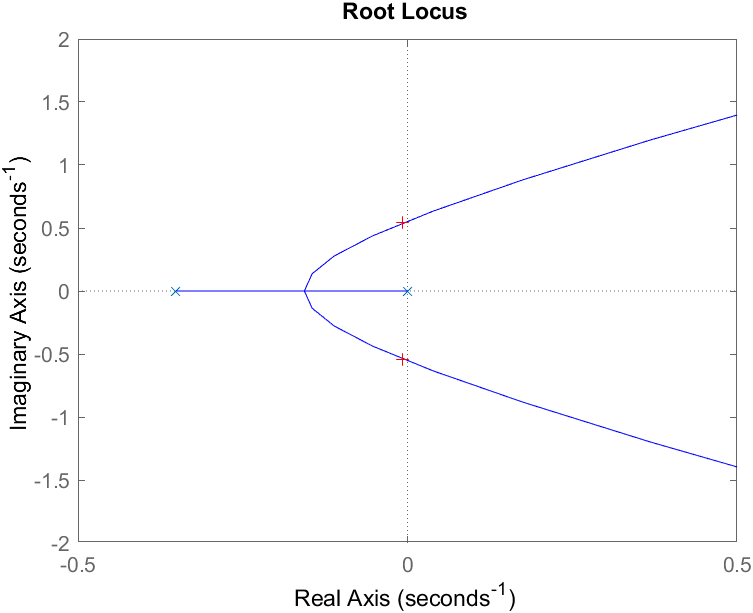
\includegraphics[width=13cm]{./img/planRacine_Kh.png}
        \caption{Lieu des racines du système\label{fig:LieuRacineKh}}
    \end{figure}



    \newpage
    \section{Énoncé 2 : Simulation}
    \subsection{Question 2.1}
    Dans le but de confirmer les plages de gains admissibles, nous allons faire varier progressivement la valeur de $K_H$ selon une fonction rampe. Cette approche permettra d'observer l'effet de l'augmentation graduelle de la rigidité sur le système, et de déterminer précisément le seuil auquel une instabilité se manifeste.
    \begin{figure}[H]
        \centering
        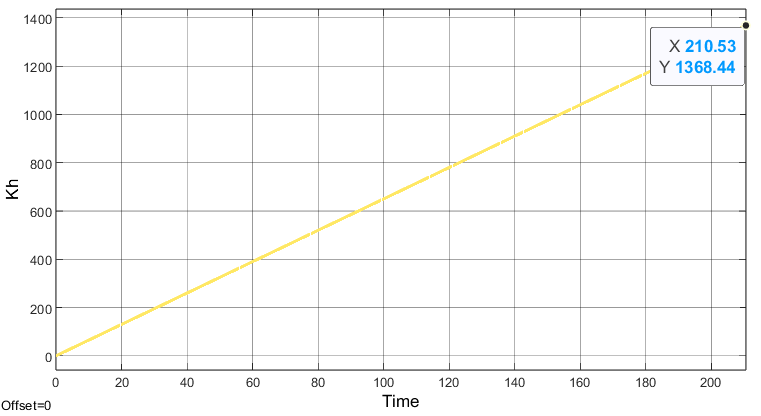
\includegraphics[width=15cm]{./img/Kh_Evolution_Rampe.png}
        \caption{Évolution de $K_H$ selon une rampe\label{fig:KhRampe}}
    \end{figure}
    
    La \autoref{fig:RespKhRampe} présente la réponse du système pour cette simulation, tandis que la \autoref{fig:KhRampe} illustre l'évolution de la rigidité $K_H$ au fil du temps. On observe que la réponse du système tend vers l'infini lorsque $K_H \approx 1368$, ce qui indique une instabilité. Cette observation permet de conclure que la plage de valeurs de $K_H$  admettant un comportement stable est $K_H \in \left< 0, 1350 \right>$.
    \begin{figure}[H]
        \centering
        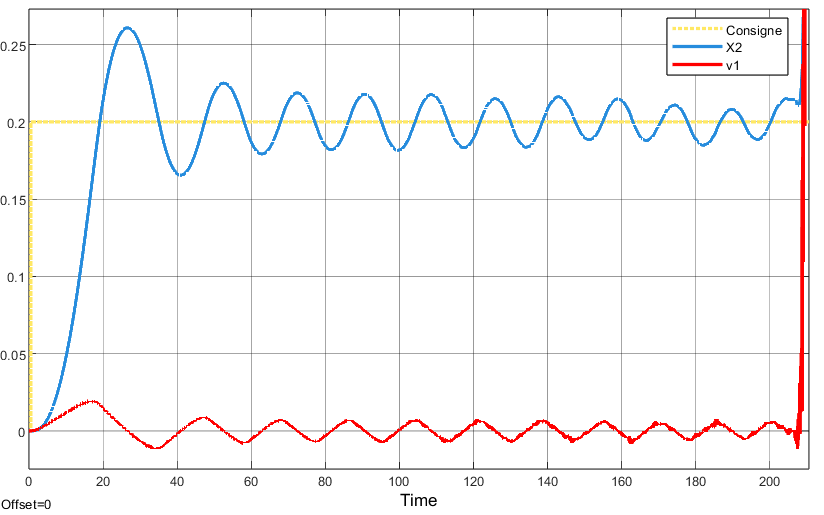
\includegraphics[width=16cm]{./img/response_KhRampe.png}
        \caption{Évolution de la réponse avec $K_H$ selon une rampe\label{fig:RespKhRampe}}
    \end{figure}
    
    
    \subsection{Question 2.2}
    Afin de confirmer la stabilité du système, on retire le modèle humain, comme le montre la \autoref{fig:SchemBlocNoHum}. Cela nous permettra d'observer le fonctionnement du système sans perturbations en entrée.
    \begin{figure}[H]
        \centering
        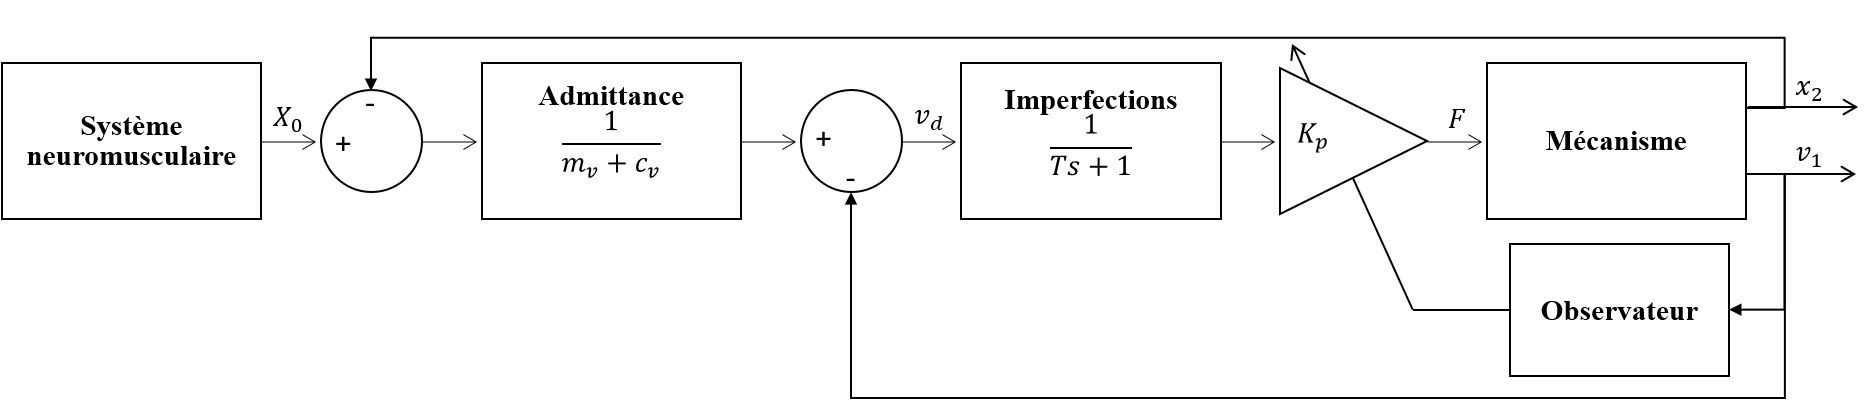
\includegraphics[width=16cm]{./img/SchemaBlocNoHum.png}
        \caption{Évolution de la réponse sans humain\label{fig:SchemBlocNoHum}}
    \end{figure}

    La réponse obtenue présente un gain (cf. \autoref{fig:RespNoHumGain}) sans oscillation, ce qui témoigne d'une stabilité satisfaisante du système. En effet, l'absence d'oscillations suggère que le système atteint son état d'équilibre sans dépasser ou fluctuer autour de la consigne, caractéristique d'un comportement stable et bien contrôlé.
    \begin{figure}[H]
        \centering
        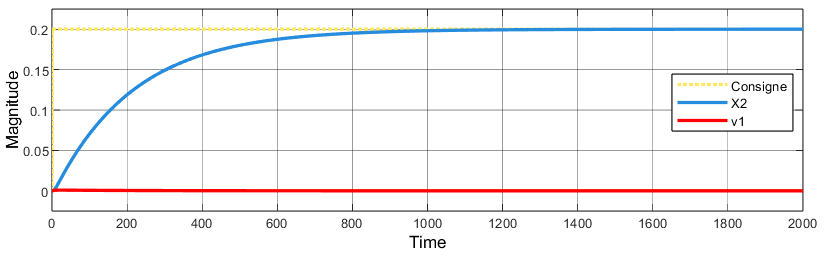
\includegraphics[width=16cm]{./img/response_NoHum_Gain.png}
        \caption{Évolution de la réponse sans humain\label{fig:RespNoHumGain}}
    \end{figure}
    
    Cette observation est renforcée par l'analyse du déphasage, illustrée dans la \autoref{fig:RespNoHumPhase}. Au cours de la simulation, aucun déphasage significatif n'est observé, ce qui confirme que la phase de la sortie suit de manière quasi-linéaire l'entrée, sans délai ou retard perceptible.
    \begin{figure}[H]
        \centering
        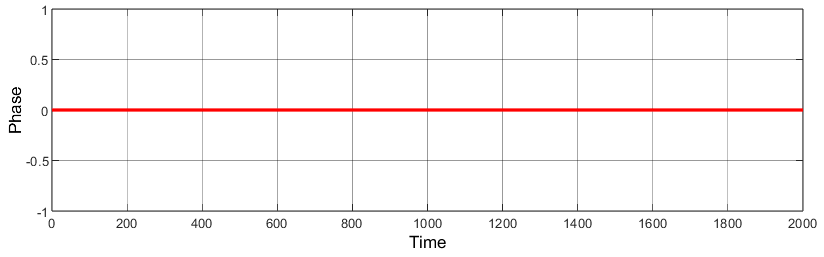
\includegraphics[width=16cm]{./img/response_NoHum_Phase.png}
        \caption{Évolution de la phase de la réponse sans humain\label{fig:RespNoHumPhase}}
    \end{figure}

    
    \subsection{Question 2.3}
    Notre dernière simulation consistera à appliquer différentes rigiditées humaine afin d'observer la réponse de notre système. Pour cela, on fait varier $K_H$ selon trois valeurs définies par trois fonctions "step" configurées tel que présenté dans l'\hyperref[Annexe:modelHumain]{annexe 5}.
    \begin{figure}[H]
        \centering
        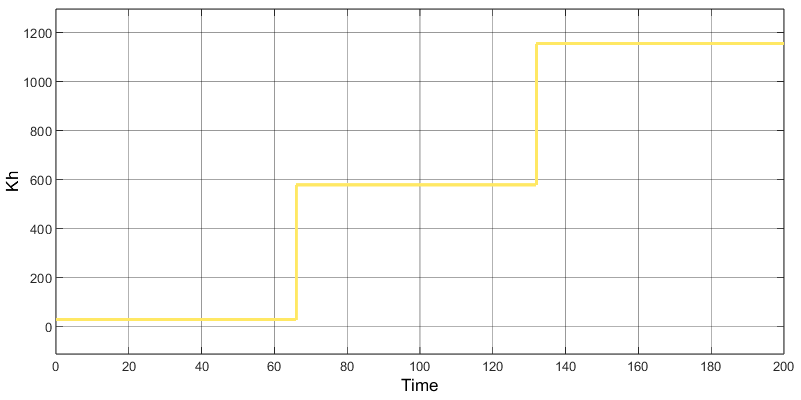
\includegraphics[width=15cm]{./img/Kh_Evolution_Steps.png}
        \caption{Évolution de $K_H$ selon trois fonctions step\label{fig:KhSteps}}
    \end{figure}

    Sur la réponse présentée dans la \autoref{fig:RespKhSteps}, on observe que l'amortissement du système est satisfaisant tant que la valeur de $K_H$ reste proche de zéro. Cependant, lors de la première augmentation de la rigidité, on note l'apparition progressive d'ondulations. Dès que $K_H$ augmente pour sa valeur finale, ces ondulations deviennent plus prononcées. De plus, des vibrations commencent à se manifester sur le signal $v_1$, qui représente la vitesse des moteurs.
    \begin{figure}[H]
        \centering
        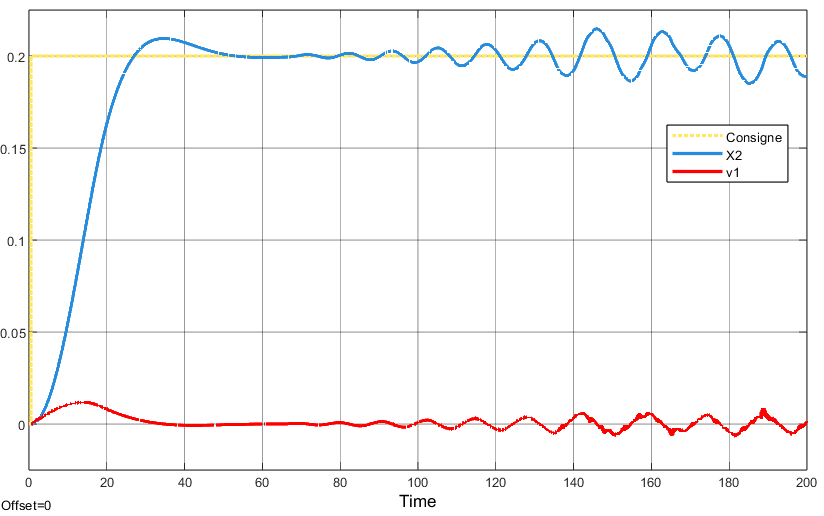
\includegraphics[width=16cm]{./img/response_KhSteps.png}
        \caption{Évolution de la réponse avec $K_H$ selon trois fonctions step\label{fig:RespKhSteps}}
    \end{figure}
    
    

    \newpage
    \section{Discussions}
    Cette étude a permis de concevoir un système de compensation des vibrations générées par la rigidité du corps humain.

    Cependant, le système présente certaines limites. En effet, il a été observé qu'au-delà d'un certain seuil de rigidité, le système rencontre des difficultés à amortir efficacement les oscillations et à compenser les vibrations. Si la rigidité continue d'augmenter, le système perd sa capacité à suivre les mouvements, ce qui conduit à une instabilité complète.

    Ces résultats soulignent qu'il est essentiel pour l'opérateur de maintenir une vigilance constante lors de l'utilisation de cet outil, notamment en veillant à limiter l'impact de la rigidité corporelle sur le système.
    
    
    \section{Conclusion}
    En conclusion, cette étude a permis de développer un système innovant destiné à améliorer la stabilité d'un dispositif asservi, en limitant l'impact des variations humaines sur sa dynamique. Ce système offre une solution prometteuse pour compenser les effets de la rigidité corporelle, contribuant ainsi à optimiser les performances du système dans des conditions d'utilisation variées.

    Après avoir validé les performances du système par simulation, la prochaine étape consistera à concevoir un prototype fonctionnel pour tester son efficacité dans des conditions réelles. Si cette phase de prototypage se révèle concluante, une phase de validation expérimentale pourra être lancée, ouvrant ainsi la voie à une commercialisation éventuelle du produit.



    \newpage
    \section{Annexes}
    \subsection{Annexe 1 : Liste des valeurs fixes} \label{Annexe:ValList}
    \begin{itemize}
        \item[] \makebox[5cm][l]{\makebox[.6cm][l]{$M_R$} = 500 $kg$} \textit{(masse de la charge)}
        \item[] \makebox[5cm][l]{\makebox[.6cm][l]{$m_R$} = 50 $kg$} \textit{(masse du système)}
        \item[] \makebox[5cm][l]{\makebox[.6cm][l]{$m_v$} = 20 $kg$} \textit{(masse ressentie)}
        \item[] \makebox[5cm][l]{\makebox[.6cm][l]{$K_B$} = 40000 $N/m$} \textit{(constante de raideur des courroies)}
        \item[] \makebox[5cm][l]{\makebox[.6cm][l]{$C_B$} = 40 $N\cdot s/m$} \textit{(coefficient d'amortissement des courroies)}
        \item[] \makebox[5cm][l]{\makebox[.6cm][l]{$C_H$} = 23.45 $N\cdot s/m$} \textit{(coefficient d'amortissement de l'humain)}
        \item[] \makebox[5cm][l]{\makebox[.6cm][l]{$C_R$} = 100 $N\cdot s/m$} \textit{(coefficient de frottement)}
        \item[] \makebox[5cm][l]{\makebox[.6cm][l]{$c_v$} = 20 $N\cdot s/m$} \textit{(coefficient d'amortissement vituel)}
        \item[] \makebox[5cm][l]{\makebox[.6cm][l]{$T$} = 0.1 $s$} \textit{(temps d'échantillonnage)}
    \end{itemize}


    \subsection{Annexe 2 : Fichier de calculs des plages de $K_p$ et $K_H$} \label{Annexe:calcRHFile}
    \begin{lstlisting}[caption={Fonction simulink de calcul du compensateur}, language=Matlab]
    % Initialisation ======================================
    close all
    system_config
    clear Kp Kh
    FontName = 'Times';

    % Calcul des boucles ==================================
    [Boucle_ouverte, Boucle] = Calc_Sys();

    % Creation de la table de Routh-Hurwitz ===============
    syms Kp Kh s
    S_boucle = calcTabRH(Boucle, [sym('MR') sym('mR') sym('Kb') sym('Cb') sym('CR') sym('T') sym('mv') sym('cv')], [MR mR Kb Cb CR T mv cv], s);

    % Recherche de la plage de valeurs Kp =================
    Kp = 0:1500;
    Kh = 50;
    figure;
    hold on
    for i = 1:length(S_boucle(:,1))
        if ~isempty(find(symvar(S_boucle(i,1)) == sym('Kp'), 1))
            S_boucle(i,1) = subs(S_boucle(i,1), sym('Kh'), Kh);
            S_calc = eval(subs(S_boucle(i,1), sym('Kp'), Kp));
    
            subplot(3, 2, i)
            plot(Kp, S_calc, 'LineWidth', 2)
            yline(0, '--')
            xlabel('Kp')
            ylabel("Critere de Routh-Hurwitz S^" + i)
            fontname(FontName)
        end
    end
    hold off
    
    % Recherche de la plage de valeurs Kh =================
    TF = subs( ...
        Boucle_ouverte, ...
        [sym('MR') sym('mR') sym('Kb') sym('Cb') sym('CR') sym('T') sym('mv') sym('cv') sym('Kp')], ...
        [MR mR Kb Cb CR T mv cv 90] ...
    );
    clear s
    TFFun = matlabFunction(TF);
    TFFun = str2func(regexprep(func2str(TFFun), '\.([/^\\*])', '$1'));
    figure;
    sys = tf(TFFun(tf('s')));
    rlocus(sys)
    axis([-0.5, 0.5, -2, 2])
    [K, poles] = rlocfind(sys);
    

    %%%%%%%%%%%%%%%%%%%%%%%%%%%%%%%%%%%%%%%%%%%%%%%%%%%%%%%
    % Parametres :                                        %
    %   (Aucun)                                           %
    % Sortie :                                            %
    %   - Boucle_NoKh : boucle ouverte                    %
    %   - Boucle1 : boucle fermee                         %
    %%%%%%%%%%%%%%%%%%%%%%%%%%%%%%%%%%%%%%%%%%%%%%%%%%%%%%%
    function [Boucle_NoKh, Boucle1] = Calc_Sys()
        syms MR mR Kb Cb CR Kh Kp T mv cv s

        % Calcul de la boucle de vitesse ==================
        BoucleVitesse0 = Kp*(MR*s^2+Kb+Cb*s+CR*s)*s*1 / (s * (mR*s^3*MR + mR*s*Kb + mR*s^2*Cb + mR*s^2*CR + Kb*MR*s + Kb*CR + Cb*s^2*MR + Cb*s*CR) * (T*s+1));
        BoucleVitesse1 = collect(simplify(BoucleVitesse0/(1+BoucleVitesse0)), s);
        
        Humain = Kh;
        Admittance = 1/(mv*s+cv);
        % Calcul de la boucle complete ====================
        Boucle0 = Humain * Admittance * BoucleVitesse1 * ((MR*s^2+Kb+Cb*s+CR*s)*s)^(-1) * (Kb+Cb*s);
        Boucle_NoKh = Admittance * BoucleVitesse1 * ((MR*s^2+Kb+Cb*s+CR*s)*s)^(-1) * (Kb+Cb*s);
        Boucle1 = collect(simplify(Boucle0*(1+Boucle0)^(-1)), s);
    end
    
    %%%%%%%%%%%%%%%%%%%%%%%%%%%%%%%%%%%%%%%%%%%%%%%%%%%%%%%
    % Parametres :                                        %
    %   - TF : la fonction de transfert a analyser        %
    %   - Oldvars : les variables a remplacer             %
    %   - Newvars : les valeurs a implementer             %
    %   - s : la variable de Laplace                      %
    % Sortie :                                            %
    %   - S : le tableau construit                        %
    %%%%%%%%%%%%%%%%%%%%%%%%%%%%%%%%%%%%%%%%%%%%%%%%%%%%%%%
    function S = calcTabRH(TF, Oldvars,  Newvars, s)
        % Extraction des coefficients du denominateur =====
        [~, Den] = numden(TF);
        [an, terms] = coeffs(Den, s);
        l_terms = length(terms);
        l = round(l_terms/2);

        % Creation du tableau =============================
        S = sym(zeros(l_terms, l));
        % Ajout des coefficients du denominateur
        for n=1:l
            i = n*2;
            S(l_terms, n) = an(i-1);
            if i < l_terms
                S(l_terms-1, n) = an(i);
            end
        end
        % Calcul des autres elements du tableau
        for k=l_terms-2:-1:1
            for n=1:l-1
                S(k, n) = (S(k+1, 1)*S(k+2, n+1)-S(k+2, 1)*S(k+1, n+1))/S(k+1, 1);
            end
        end

        % Remplacement des valeurs connues ================
        S = simplify(subs(S, Oldvars, Newvars));

        % Affichage du tableau ============================
        disp("Tableau du critere de Routh-Hurwitz :")
        disp(S)
    end
    \end{lstlisting}


    \subsection{Annexe 3 : Fichier de configuration de la simulation} \label{Annexe:configSimu}
    \begin{lstlisting}[caption={Fonction simulink de calcul du compensateur}, language=Matlab]
    clear;
    clc;

    %Temps de simulation
    sim_time = 200;     % s
    % Taille de la memoire tampon de l'observateur
    buffer_size = 128;

    % Bloc "Modele humain" ================================
    Kh = 550;           % N/m
    Ch = 23.45;         % N*s/m
    
    % Admittance ==========================================
    cv = 20;            % N*s/m
    mv = 20;            % kg
    
    % Imperfections =======================================
    T = .1;             % s

    % Mecanisme ===========================================
    mR = 50;            % kg
    MR = 500;           % kg
    CR = 100;           % N*s/m
    Cb = 40;            % N*s/m
    Kb = 40000;         % N/m
    [A, B, C, D] = calcIAD(Kb, Cb, CR, mR, MR);

    % Observateur =========================================
    % Ecart-type limite avant vibrations
    ec_max = 1e-3;

    
    %%%%%%%%%%%%%%%%%%%%%%%%%%%%%%%%%%%%%%%%%%%%%%%%%%%%%%%
    % Parametres :                                        %
    %   - K : ici Kb                                      %
    %   - C1 : ici Cb                                     %
    %   - C2 : ici CR                                     %
    %   - m : ici mR                                      %
    %   - M : ici MR                                      %
    % Sortie :                                            %
    %   - A : la matrice d'etat                           %
    %   - B : la matrice de commande                      %
    %   - C : la matrice d'observation                    %
    %   - D : la matrice d'action directe                 %
    %%%%%%%%%%%%%%%%%%%%%%%%%%%%%%%%%%%%%%%%%%%%%%%%%%%%%%%
    function [A, B, C, D] = calcIAD(K, C1, C2, m, M)
        mK = K / m;
        mC = C1 / m;
        MK = K / M;
    
        A = [
             0      0       1       0;
             0      0       0       1;
            -mK     mK      -mC     mC;
             MK     -MK     C1/M    -(C1+C2)/M
            ];
        B = [
             0;
             0;
             1/m;
             0
            ];
        C = [
             0      1       0       0;
             0      0       1       0;
            ];
        D = zeros(2, 1);
    end
    \end{lstlisting}


    \subsection{Annexe 4 : Modèle complet} \label{Annexe:modelComplet}
    \begin{center}
        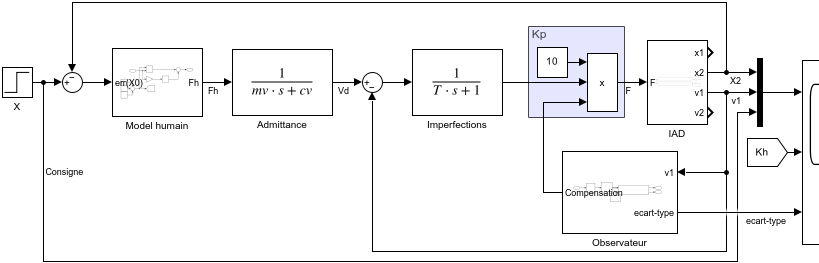
\includegraphics[width=24cm, angle=-90]{./img/model_complet.png}
    \end{center}
    Où le bloc "step" (\textbf{X}) est paramétré avec : 
    \begin{itemize}
        \item[$\bullet$] \makebox[2.3cm][l]{"step time"} = 0.5
        \item[$\bullet$] \makebox[2.3cm][l]{"initial value"} = 0
        \item[$\bullet$] \makebox[2.3cm][l]{"final value"} = 0.2
    \end{itemize}


    \subsection{Annexe 5 : Modèle humain} \label{Annexe:modelHumain}
    \begin{center}
        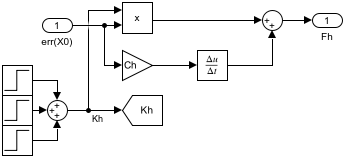
\includegraphics[width=13cm]{./img/model_humain.png}
    \end{center}
    Où :
    \begin{itemize}
        \item[] Le bloc "rate transition" est paramétré avec : 
            \subitem $\bullet$ \makebox[4.2cm][l]{"slope"} = 6.5
            \subitem $\bullet$ \makebox[4.2cm][l]{"start time"} = 0
            \subitem $\bullet$ \makebox[4.2cm][l]{"initial output"} = 0
        \item[] Et les blocs "step" sont paramétrés avec :
    \end{itemize}
    \begin{tabular*}{1\linewidth}{@{\extracolsep{\fill}}l l l}
        \hline
        \multicolumn{1}{c}{Step haut} & \multicolumn{1}{c}{Step milieu} &\multicolumn{1}{c}{Step bas} \\
        \hline
    
        $\bullet$ \makebox[2.3cm][l]{"step time"} = 0 &
        $\bullet$ \makebox[2.3cm][l]{"step time"} = 66 &
        $\bullet$ \makebox[2.3cm][l]{"step time"} = 132 \\
        
        $\bullet$ \makebox[2.3cm][l]{"initial value"} = 0 & 
        $\bullet$ \makebox[2.3cm][l]{"initial value"} = 0 & 
        $\bullet$ \makebox[2.3cm][l]{"initial value"} = 0 \\
        
        $\bullet$ \makebox[2.3cm][l]{"final value"} = 27.5 &
        $\bullet$ \makebox[2.3cm][l]{"final value"} = 550 &
        $\bullet$ \makebox[2.3cm][l]{"final value"} = 577.5 \\
    \end{tabular*}
    

    \subsection{Annexe 6 : Modèle IAD} \label{Annexe:modelIAD}
    \begin{center}
        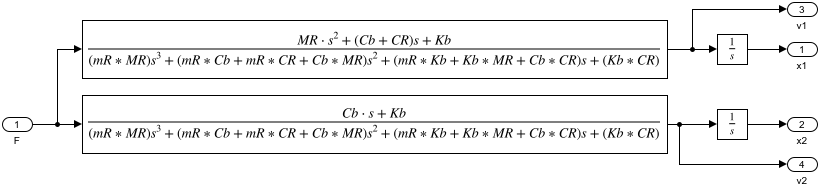
\includegraphics[width=16cm]{./img/model_IAD.png}
    \end{center}
    

    \subsection{Annexe 7 : Modèle observateur} \label{Annexe:modelObs}
    \begin{center}
        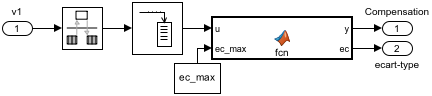
\includegraphics[width=14cm]{./img/model_observateur.png}
    \end{center}
    Où :
    \begin{itemize}
        \item[] Le bloc "rate transition" est paramétré avec : 
            \subitem $\bullet$ \makebox[4.2cm][l]{"initial conditions"} = 0
            \subitem $\bullet$ \makebox[4.2cm][l]{"ouput port sample time"} = 0.01
        \item[] Le bloc "buffer" est paramétré avec : 
            \subitem$\bullet$ \makebox[5.5cm][l]{"ouput buffer size (per channel)"} = 128
            \subitem$\bullet$ \makebox[5.5cm][l]{"buffer overlap"} = 64
            \subitem$\bullet$ \makebox[5.5cm][l]{"initial conditions"} = 0
        \item[] Et le bloc "MATLAB Function" contient :
    \end{itemize}
    \begin{lstlisting}[caption={Fonction simulink de calcul du compensateur}, language=Matlab]
    %%%%%%%%%%%%%%%%%%%%%%%%%%%%%%%%%%%%%%%%%%%%%%%%%%%%%%%
    % Parametres :                                        %
    %   - u : segment de signal                           %
    %   - ec_max : ecart-type limite avant vibration      %
    % Sortie :                                            %
    %   - y : le coefficient de compensation              %
    %   - ec : l'ecart-type du segment                    %
    %%%%%%%%%%%%%%%%%%%%%%%%%%%%%%%%%%%%%%%%%%%%%%%%%%%%%%%
    function [y, ec] = fcn(u, ec_max)
        % Calcul de l'ecart-type ==========================
        ec = std(u);

        % Calcul de la compensation =======================
        y = 1 - ec * (1/ec_max);
    end
    \end{lstlisting}
    
    
    \subsection{Lien vers le Dépôt GitHub}
    \url{https://github.com/BlueWan14/Cours_IHR/tree/main/Devoir_2}



    \newpage
    \printbibliography
\end{document}
